\section{領域ネスティング実験} \label{sec:nest_exp}
%====================================================================================

本節では、SCALEでネスティング実験を行う方法について説明する。ネスティング実験とは、図\ref{fig_nestsample}に
示すように、水平格子間隔の異なる複数の計算領域(ドメイン)を設定し、領域が重複するように入れ子(ネスト)構造に
することで、広領域かつ高解像度の領域を設定する計算領域設定方法である。図\ref{fig_nestsample}の例では、
3つの領域を用いた3段ネスティング構成になっている。外側の領域は比較的粗い
水平解像度であるが広い領域を取ることで大きな場の構造を表現することができる。逆に内側の領域は、比較的狭い
領域であるが細かい水平解像度を取ることで対象とする現象の細かい構造を表現することができる。ここでは、
入れ子構造のうち、データを渡す側の領域を「親領域」、データを受ける側の領域を「子領域」と称する。

SCALEはオフライン・ネスティング実験とオンライン・ネスティング実験の両方をサポートしている。オフライン・ネスティング実験は、
はじめに親領域だけで時間積分を行い、その計算結果のヒストリーデータを用いて、子領域用の初期値・境界値を作成する。
その後に子領域の時間積分を行う。オンライン・ネスティング実験は、親領域と子領域を同時に実行し、適宜計算途中の
データを親領域から子領域へMPI通信によって受け渡しすることで、子領域の時間積分を行う。
オンライン・ネスティング実験が実行できる計算機リソースがあれば、オンラインで実行することを推奨する。
それは、オンラインの場合、子領域の境界条件の更新間隔は親領域の時間積分間隔に一致するため、
可能な限り細かい境界条件の更新間隔を得ることができる。


オフラインネスティング実験を行う上での実験設定の制限事項は、以下の2点である。
\textcolor{red}{
\begin{itemize}
 \item 親領域の領域は子領域の領域を完全に内包しなければならない。
 \item 親領域の積分時間は子領域の積分時間を完全に内包しなければならない。
\end{itemize}
}

これに加えて、オンライン・ネスティング実験の場合、現在のところ親領域と子領域の積分時間は一致している必要があり、かつ、親領域の時間ステップは子領域の時間ステップの倍数でなければならない。
SCALEではオンライン・ネスティングであっても、親領域と子領域の間で鉛直層数、鉛直層設定、地図投影法、そして
物理スキームが異なっていても構わない。

オフライン、オンラインに関わらず、領域間の格子間隔比率($DX_{parent}/DX_{child}$)にシステム上は制限はないが、
この比率が大きすぎると計算結果の物理的なパフォーマンスが下がる可能性がある。本書では5倍以下で使用することを推奨する。

以降、まずは実行方法がわかりやすいオフライン・ネスティング実験から説明し、ついでオンライン・ネスティング実験に
ついて説明する。設定ファイルの名前に特に指定はないが、ここでの表記としては、
\textcolor{blue}{``***.parent.conf''と表記すれば、親領域の設定ファイルを編集する}ことを意味し、
\textcolor{blue}{``***.child.conf''と表記すれば、子領域の設定ファイルを編集する}ことを意味する。


\begin{figure}[t]
\begin{center}
  
\includegraphics[width=1.0\hsize]{./figure/nesting_sample.eps}\\
  \caption{日本の近畿地方を対象領域とした領域ネスティング設定の例. domain 1が最外領域でdomain 3が最内領域である。
           赤い矩形と線は、それぞれの位置関係を示している。domain 1の水平格子間隔は7.5 km、domain 2は2.5 km、
           そしてdomain 3は0.5 kmである。}
  \label{fig_nestsample}
\end{center}
\end{figure}


\subsection{オフライン・ネスティング実験の方法} \label{sec:nest_offline}
%------------------------------------------------------

ここでは、親領域は解像度は粗いが広領域の外側領域で、子領域は領域は狭いが高解像度の内側領域で
あることを想定する。このとき、2段ネスティングのオフライン・ネスティング実験の実行過程は次のようになる。

{\gt
\begin{enumerate}
 \item 親領域の時間積分計算を行う。
 \item 親領域の出力ファイル(ヒストリー)を用いて子領域の初期値/境界値を作成する。
 \item 作成した初期値/境界値を用いて子領域の時間積分計算を行う。
\end{enumerate}
}

以下、この流れに沿って説明を進める。親領域と子領域それぞれについて、``pp.***.conf''、``init.***.conf''、
そして``run.***.conf''ファイルを事前に作成し、親領域、子領域ともに地形/土地利用データの作成を終え、
親領域については、初期値/境界値データの作成を終えていることを想定して説明を進める。
ここで説明するオフライン・ネスティング実験の設定を記述した設定ファイルがチュートリアルディレクトリの下、
``tutorial/real/sample/offline\_nesting''に置いてあるので、説明を読み進める上で参考にしてもらいたい。

\subsubsection{親領域の時間積分計算を行う}
基本的には通常のシングル領域の計算と同じ方法で実行すればよいが、``run.conf''ファイルの設定について、
次の5点の注意点・変更点がある。

\begin{itemize}
 \item 親領域のヒストリー出力間隔を適度に細かくとること。
 \item 親領域のヒストリー出力変数に必要なものが揃っているか確認すること。
 \item 親領域のヒストリー出力形式で\verb|ZINTERP|は``false''に設定すること。
 \item 親領域のヒストリー出力形式で\verb|STEP0|は``true''に設定すること。
 \item 親領域の計算領域を子領域へ伝える「カタログファイル」を出力すること。
\end{itemize}


この設定を``run.parent.conf''に適用すると下記のようになる。赤文字で示した部分が、
上記の注意点・変更点に対応する部分である。\\

\noindent {\small {\gt
\ovalbox{
\begin{tabularx}{140mm}{l}
\textcolor{red}{\verb|&PARAM_DOMAIN_CATALOGUE|} \\
\textcolor{red}{\verb| DOMAIN_CATALOGUE_OUTPUT = .true.,|} \\
\textcolor{red}{\verb|/|} \\
 \\
\verb|&PARAM_HISTORY| \\
\verb| HISTORY_DEFAULT_BASENAME  = "history",| \\
\textcolor{red}{\verb| HISTORY_DEFAULT_TINTERVAL = 600.D0,|} \\
\verb| HISTORY_DEFAULT_TUNIT     = "SEC",| \\
\verb| HISTORY_DEFAULT_TAVERAGE  = .false.,| \\
\verb| HISTORY_DEFAULT_DATATYPE  = "REAL4",| \\
\textcolor{red}{\verb| HISTORY_DEFAULT_ZINTERP   = .false.,|} \\
\textcolor{red}{\verb| HISTORY_OUTPUT_STEP0      = .true.,|} \\
\verb|/| \\
\end{tabularx}
}}}\\

\verb|PARAM_DOMAIN_CATALOGUE|の項目の``\verb|DOMAIN_CATALOGUE_OUTPUT|''の変数がカタログファイルの出力設定である。
もともとの設定ファイルには項目自体がないこともあるので、その場合は自分で項目を加えて設定すること。
カタログファイルは、``latlon\_domain\_catalogue.txt''というファイル名で出力される。この中には、MPIプロセス毎に分割
して担当した計算領域の四隅の緯度・経度が記述されている。

\verb|HISTORY_DEFAULT_TINTERVAL|の設定項目によってヒストリーデータ出力間隔を指定する(単位は秒である)。指定値に
任意性はあるが、子領域の側面境界条件の更新間隔として使用可能であると考えられる範囲で指定すること。
親領域、子領域の解像度、および実行環境のディスク空き容量にもよるが、おおよそ最大で1時間間隔、
出来れば10分間隔のヒストリーデータ出力間隔を指定することが多い。

また、ヒストリーデータを用いて初期値/境界値データを作成するために、
下記の全ての変数を出力する必要がある。
run.confファイルの``HISTITEM''の項目を確認すること。

\begin{itemize}
 \item \verb|T2, Q2, MSLP, DENS, MOMZ, MOMX, MOMY, RHOT|
 \item \verb|QV, QC, QR, QI, QS, QG| {\small (親の雲微物理モデルに合わせて出力; 例えばTomita08なら全て)}
 \item \verb|NC, NR, NI, NS, NG| {\small (親の雲微物理モデルに合わせて出力; 例えばTomita08なら不要)}
 \item \verb|LAND_SFC_TEMP, URBAN_SFC_TEMP, OCEAN_SFC_TEMP|
 \item \verb|OCEAN_ALB_LW, OCEAN_ALB_SW, LAND_ALB_LW, LAND_ALB_SW|
 \item \verb|OCEAN_TEMP, OCEAN_SFC_Z0M, LAND_TEMP, LAND_WATER|
\end{itemize}

設定が完了すれば、``scale-rm''を実行して親領域の時間積分計算を行う。


\subsubsection{親領域の出力ファイルを用いて子領域の初期値/境界値を作成する}
次に計算が終わった親領域のヒストリーデータ出力を用いて、子領域の初期値/境界値を作成する。
実行するプログラムは、通常の初期値/境界値作成と同じ``scale-rm\_init''だが、
``init.child.conf''を下記のように編集する。\\

\noindent {\small {\gt
\ovalbox{
\begin{tabularx}{140mm}{l}
\verb|&PARAM_MKINIT_REAL| \\
\verb| BASENAME_BOUNDARY   = "boundary",| \\
\textcolor{red}{\verb| BASENAME_ORG        = "history",|} \\
\textcolor{red}{\verb| FILETYPE_ORG        = "SCALE-RM",|} \\
\textcolor{red}{\verb| NUMBER_OF_TSTEPS    = 25,|} \\
\textcolor{red}{\verb| BOUNDARY_UPDATE_DT  = 600.D0,|} \\
\verb|/| \\
 \\
\textcolor{red}{\verb|&PARAM_NEST|} \\
\textcolor{red}{\verb| USE_NESTING               = .true.,|} \\
\textcolor{red}{\verb| OFFLINE                   = .true.,|} \\
\textcolor{red}{\verb| OFFLINE_PARENT_PRC_NUM_X  = 4,|} \\
\textcolor{red}{\verb| OFFLINE_PARENT_PRC_NUM_Y  = 4,|} \\
\textcolor{red}{\verb| OFFLINE_PARENT_KMAX       = 35,|} \\
\textcolor{red}{\verb| OFFLINE_PARENT_IMAX       = 40,|} \\
\textcolor{red}{\verb| OFFLINE_PARENT_JMAX       = 40,|} \\
\textcolor{red}{\verb| OFFLINE_PARENT_LKMAX      = 5,|} \\
\textcolor{red}{\verb| LATLON_CATALOGUE_FNAME    = "latlon_domain_catalogue.txt",|} \\
\textcolor{red}{\verb|/|} \\
\end{tabularx}
}}}\\

\noindent 読み込む外部入力データのファイル名を指定する``\verb|BASENAME_ORG|''は、親モデルのhistory.pe***.nc
ファイルを読み込むので、``history''と指定する。また、このヒストリーファイルはSCALE-RMモデルの出力データなので、
``\verb|FILETYPE_ORG|''は、``SCALE-RM''と指定する。\verb|NUMBER_OF_TSTEPS|には、ヒストリーファイルが持つ時間ステップ数
を記述する(例として25が記述されているだけ)。\verb|BOUNDARY_UPDATE_DT|には、時間ステップの時間間隔を指定する
(単位は秒である)。つまり、親領域の\verb|HISTORY_DEFAULT_TINTERVAL|の設定項目に一致する値を指定する。
この説明では、親領域で600秒としたので、ここでも600秒を指定する。

\verb|PARAM_NEST|の項目は、ネスティング実験のために新たに加える項目である。もともとの設定ファイルには項目自体がないので、
自分で設定ファイルに追記する。最初の2つの項目によって、オフライン・ネスティング実験であることが決定される。
``\verb|OFFLINE_PARENT_|''で始まる6つの設定変数は、親領域の設定を記述する変数である。親領域の対応する項目を
参照して正しく設定すること。この例では、親領域は$4 \times 4$のMPIプロセス数を使用し、鉛直35層で、水平には1つの
MPIプロセスあたり$40 \times 40$の格子点を持っており、陸面モデルは5層モデルであることを想定している。
最後の``\verb|LATLON_CATALOGUE_FNAME|''の項目は、親領域を実行した時に出力したカタログファイルを指定する。

設定の編集が完了すれば、``scale-rm\_init''を実行して子領域の初期値/境界値を作成する。\\

\noindent {\small {\gt
\fbox{
\begin{tabularx}{140mm}{l}
\verb|xxx ERROR: REQUESTED DOMAIN IS TOO MUCH BROAD| \\
\verb|xxx -- LONGITUDINAL direction over the limit| \\
\end{tabularx}
}}}\\

\noindent 実行時に上記のようなメッセージが表示されて計算が止まる場合は、子領域の計算領域が親領域の計算領域の
外側に取られている部分がある。この場合は、各領域の大きさや領域中心の設定を見直す必要がある。


\subsubsection{作成した初期値/境界値を用いて子領域の時間積分計算を行う}
初期値/境界値作成が終われば、子領域の時間積分計算を実行する。子領域の実行は、通常の現実大気実験と何も変わらないので、
必要なデータのPATHが正しく設定ファイルに記述されていることを確認してから、``scale-rm''を実行すればよい。

1点だけ忘れやすい設定項目を挙げておく。\\

\noindent {\small {\gt
\ovalbox{
\begin{tabularx}{140mm}{l}
\verb|&PARAM_MKINIT_REAL| \\
\verb|     〜 中略 〜|\\
\textcolor{red}{\verb| BOUNDARY_UPDATE_DT  = 600.D0,|} \\
\verb|/| \\
\end{tabularx}
}}}\\

\noindent ``run.child.conf''の\verb|BOUNDARY_UPDATE_DT|を、初期値/境界値作成で使用した親領域の
ヒストリーデータ出力間隔に合わせておくことを忘れないようにすること。オフライン・ネスティング実験の場合、
現在のところこの設定に親領域と子領域間で不整合あっても警告やエラーメッセージが発せられないまま、
時間積分計算が進み、場合によっては正常終了してしまうため注意が必要である。

多段のオフライン・ネスティング実験を行いたい場合は、ここまでの過程を繰り返せばよい。つまり、子領域として
時間積分計算した結果を再度、親領域と見立てて、さらに内側の孫領域の初期値/境界値作成を行なえばよい。
以上でオフライン・ネスティングの実行方法の説明を終える。


\subsection{オンライン・ネスティング実験の方法} \label{sec:nest_online}
%------------------------------------------------------

オフライン・ネスティング実験では、各領域の計算を逐次的に実行する必要があったが、オンライン・ネスティング実験では
全ての領域の計算を同時に実行する。現在は、親領域から子領域へのみデータ受け渡しを行う、いわゆる
``1-wayネスティング''のみをサポートしている。オンライン・ネスティング実験でサポートするネスティング段数は、
最大で10段までである。

SCALEのオンライン・ネスティング実験は、複数の領域を逐次的に時間積分計算を進めるのではなく、並列的に時間積分計算を行う。
図\ref{fig_mpisplit}に示すイメージ図のように、与えられたMPIプロセスを分割してそれぞれの領域に分配し、各々の領域が
独立したモデルのように計算を進める。後ほど説明するが、複数の領域を立ち上げるために実行時には``launch.conf''という
起動用の設定ファイルが別途必要になる。

\begin{figure}[t]
\begin{center}
  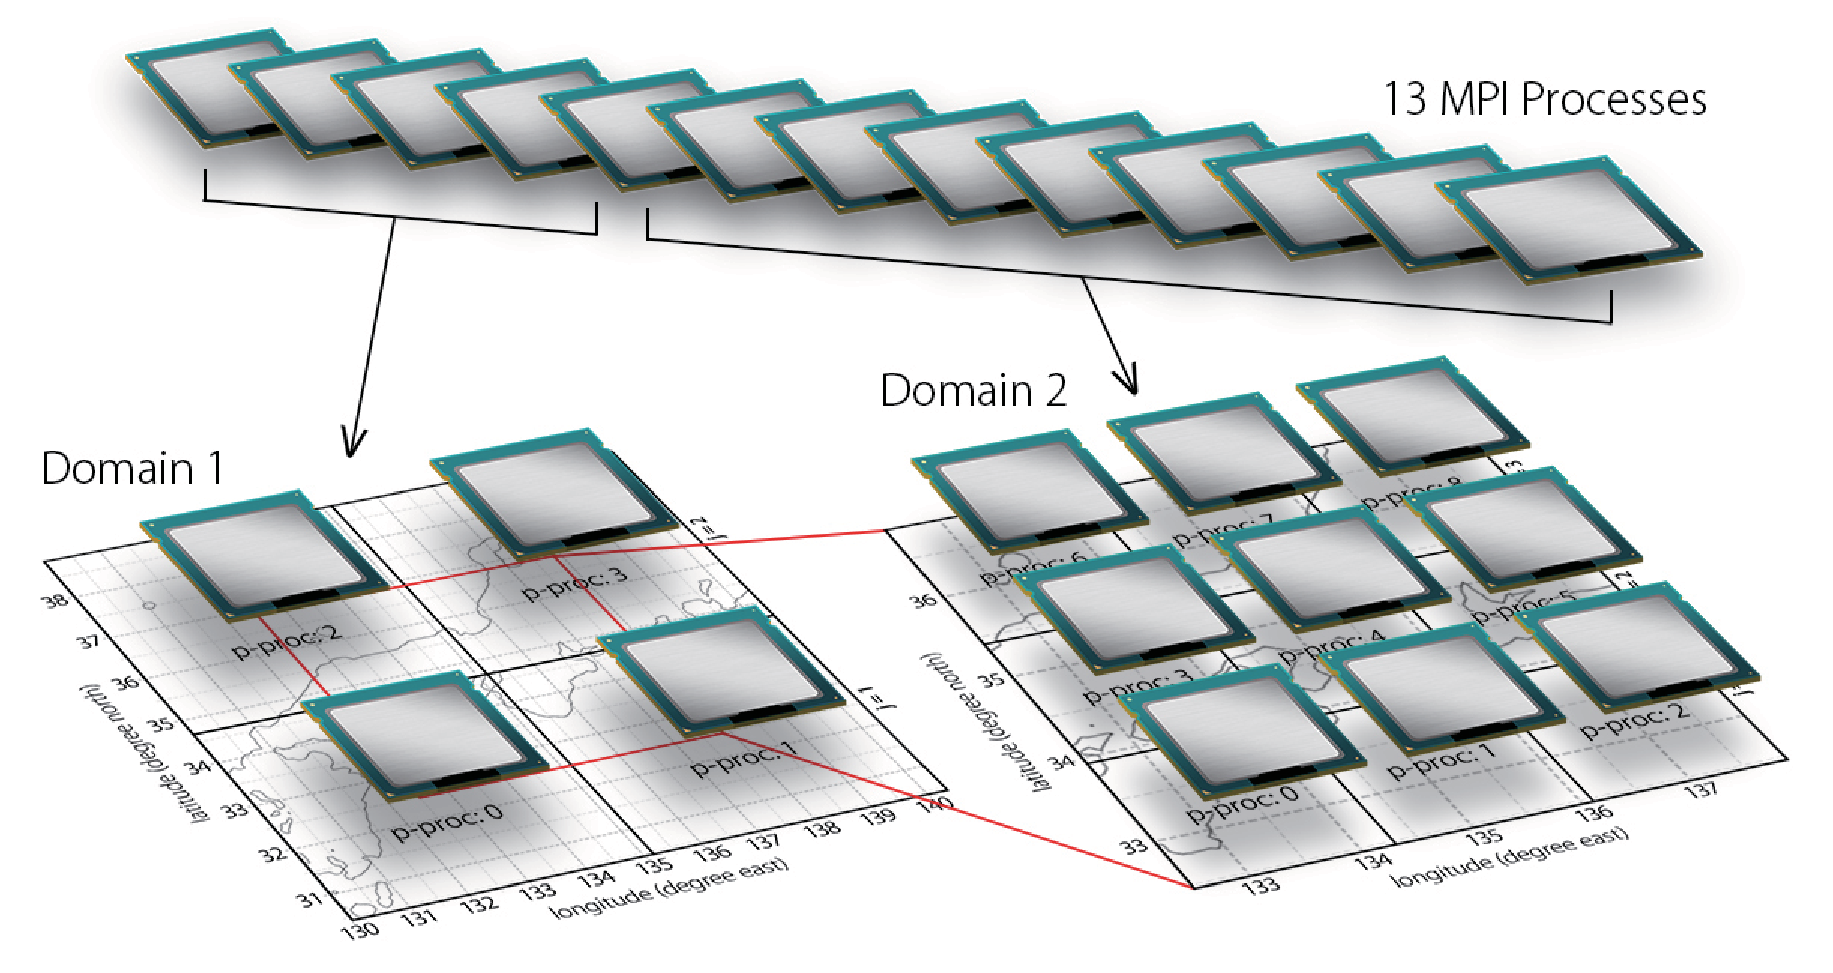
\includegraphics[width=0.8\hsize]{./figure/mpisplit_nesting.eps}\\
  \caption{オンライン・ネスティング実験のMPIプロセス配分イメージ. 全部で13のプロセスを立ち上げ、これを適切に分配することで、
           Domain 1は$2 \times 2$の4-MPI並列、Domain 2は$3 \times 3$の9-MPI並列計算を行う。Domain 1からDomain 2へMPI通信
           によってデータを受け渡ししながら時間積分計算を進める。}
  \label{fig_mpisplit}
\end{center}
\end{figure}


ここでは、最も単純な2段ネスティングの例を説明する。親領域は解像度は粗いが広領域の外側領域で、
子領域は領域は狭いが高解像度の内側領域であることを想定する。

オンライン・ネスティング実験を行う場合は、``scale-rm''のモデル本体実行前に全ての領域について、
地形/土地利用データの作成、及び初期値/境界値データの作成を事前に行っておく必要がある。従って、親領域と子領域
それぞれについて、``pp.***.conf''、``init.***.conf''、そして``run.***.conf''ファイルを事前に作成し、
親領域、子領域ともに地形/土地利用データの作成、及び初期値/境界値データの作成を終えていることを想定して説明を進める。
ここで説明するオンライン・ネスティング実験の設定を記述した設定ファイルがチュートリアルディレクトリの下、
``tutorial/real/sample/online\_nesting''に置いてあるので、説明を読み進める上で参考にしてもらいたい。


\subsubsection{設定ファイルの編集}
まず、親領域、子領域それぞれに``run.***.conf''ファイルを編集する。

\noindent {\gt \verb|run.parent.conf|の編集内容}\\
{\small {\gt
\ovalbox{
\begin{tabularx}{140mm}{l}
\verb|&PARAM_NEST| \\
\verb| USE_NESTING              = .true.,| \\
\verb| OFFLINE                  = .false.,| \\
\verb| ONLINE_DOMAIN_NUM        = 1,| \\
\verb| ONLINE_IAM_PARENT        = .true.,| \\
\verb| ONLINE_IAM_DAUGHTER      = .false.,| \\
\verb| ONLINE_BOUNDARY_USE_QHYD = .true.,| \\
\verb| ONLINE_AGGRESSIVE_COMM   = .true.,| \\
\verb|/| \\
\end{tabularx}
}}}\\

\vspace{0.5cm}

\noindent {\gt \verb|run.child.conf|の編集内容}\\
{\small {\gt
\ovalbox{
\begin{tabularx}{140mm}{l}
\verb|&PARAM_NEST| \\
\verb| USE_NESTING              = .true.,| \\
\verb| OFFLINE                  = .false.,| \\
\verb| ONLINE_DOMAIN_NUM        = 2,| \\
\verb| ONLINE_IAM_PARENT        = .false.,| \\
\verb| ONLINE_IAM_DAUGHTER      = .true.,| \\
\verb| ONLINE_BOUNDARY_USE_QHYD = .true.,| \\
\verb| ONLINE_AGGRESSIVE_COMM   = .true.,| \\
\verb|/| \\
\end{tabularx}
}}}\\

\noindent 上記の\verb|PARAM_NEST|の項目は、ネスティング実験のために新たに加える項目である。
もともとの設定ファイルには項目自体がないので、自分で設定ファイルに追記する。最初の2つの項目によって、
オンライン・ネスティング実験であることが決定される。``\verb| ONLINE_|''で始まる設定変数はオンライン・ネスティング実験
専用の設定変数である。\verb|ONLINE_DOMAIN_NUM|は、領域のID番号であり、外側領域から内側領域へ順番に
番号を振っていく。ここでは、親領域は1番、子領域は2番と設定する。

\verb|ONLINE_IAM_PARENT|と\verb|ONLINE_IAM_DAUGHTER|は各領域の役割を設定するパラメータである。
これらの変数は、``In online nesting system, I am parent (or, I am child).''という意味で覚えれば設定を間違うことはない。
少し脇道にそれるが、ここで説明している設定より複雑なものとして、図\ref{fig_nestsample}のような
3段ネスティング実験の場合の設定例を表\ref{tab:triple_nested}に示した。

\begin{table}[htb]
\begin{center}
\caption{3段ネスティング実験の設定例}
\begin{tabularx}{150mm}{|l|l|l|X|} \hline
 \rowcolor[gray]{0.9} 領域 & \verb|ONLINE_DOMAIN_NUM| & \verb|ONLINE_IAM_PARENT| & \verb|ONLINE_IAM_CHILD|\\ \hline
 最外領域 & 1 & \textcolor{blue}{true} & \textcolor{red}{false} \\ \hline
 中間領域 & 2 & \textcolor{blue}{true} & \textcolor{blue}{true} \\ \hline
 最内領域 & 3 & \textcolor{red}{false} & \textcolor{blue}{true} \\ \hline
\end{tabularx}
\label{tab:triple_nested}
\end{center}
\end{table}

\noindent 最外領域は親領域としてのみ働き、最内領域は子領域としてのみ働く。一方、中間領域は最外領域に
対しては子領域、最内領域に対しては親領域として働くため両方共``true''となる。

さて、設定ファイルの編集内容の説明に戻る。\verb|ONLINE_BOUNDARY_USE_QHYD|は、「側面境界条件として親領域の凝結物の
混合比を使うかどうか」を指定する設定変数である。外部入力データから側面境界条件を作成するときには通常使わないが、
ネスティングの場合、領域間の物理スキームの違いがなかったり、解像度もそれほど大きく離れていないため、側面境界から
凝結物自体が移流して入ってくる設定も選択肢に入るだろう。側面境界付近で雲が立ちにくい問題を解決したり、親領域との乖離を
抑制したりする可能性がある。

最後の\verb|ONLINE_AGGRESSIVE_COMM|はオンライン・ネスティング時の領域間通信に関する最適化変数である。
通常は、``true''と設定して実行する。


\subsubsection{launchファイルの編集}
オンライン・ネスティング実験の実行には、``run.***.conf''の他に、起動用設定ファイル``launch.conf''が必要である。
\begin{verbatim}
 $ vi launch.conf
\end{verbatim}
などとして、適宜エディタをたちあげて新規ファイルを作成し、下記の内容を記述する。\\

\noindent {\small {\gt
\ovalbox{
\begin{tabularx}{140mm}{l}
\verb|&PARAM_LAUNCHER| \\
\verb| NUM_DOMAIN  = 2,| \\
\verb| CONF_FILES  = run.parent.conf,run.child.conf,| \\
\verb| PRC_DOMAINS = 4,9,| \\
\verb|/| \\
\end{tabularx}
}}}\\

\noindent 図\ref{fig_mpisplit}のイメージを思い浮かべながら設定を確認してもらいたい。\verb|PARAM_LAUNCHER|の項目のうち、
\verb|NUM_DOMAIN = 2|が「2つの領域を起動する」ことを表しており、\verb|CONF_FILES|の項目に羅列されたファイル名は、
各々の領域で読み込む設定ファイルを指定している。\verb|PRC_DOMAINS|は各々の領域で使用するMPIプロセス数を
指定する。\verb|PRC_DOMAINS|は、\verb|CONF_FILES|で羅列した順番で指定しなければならない。従ってこの場合、
親領域は4-MPI並列、子領域は9-MPI並列で実行するように指定されている。ここで指定するMPIプロセス数は、
各々の``run.***.conf''で指定されている総MPIプロセス数と合致させなければならない。
この2段オンライン・ネスティング実験で使用する総MPIプロセス数は、$4 + 9 = 13$プロセスとなる。

実行時には、シングル領域計算とは異なり、\verb|launch.conf|を引数に指定し、計算全体で使用するMPIプロセス数を
指定して実行する。
\begin{verbatim}
 $ mpirun  -n  13  ./scale-rm  launch.conf
\end{verbatim}

実行にあたって注意することは、複数の領域の計算を同時に実行するため、\textcolor{red}{領域間で設定ファイルに
記述された出力ファイル名を領域毎に変更しなければならない}ことである。たとえば,``history.pe***.nc''は、
``history\_d01.pe***.nc''、``history\_d02.pe***.nc''といったように領域毎に名前を変えながらどの領域の
出力データであるか判別がつくように設定ファイルの記述を設定する。
ヒストリーファイルのほかに、LOGファイル、topoファイル、landuseファイル、boundaryファイル、initファイル、restartファイル、
そしてmonitorファイルの名前を変更しておく必要がある。

実行時に次のようなエラーメッセージが出力されて計算が異常終了することがある。\\

\noindent {\small {\gt
\fbox{
\begin{tabularx}{140mm}{l}
\verb|xxx region of daughter domain is larger than that of parent: SW search| \\
\end{tabularx}
}}}\\

\noindent {\small {\gt
\fbox{
\begin{tabularx}{140mm}{l}
\verb|xxx region of daughter domain is larger than that of parent: NE search| \\
\end{tabularx}
}}}\\

\noindent これは、子領域で設定された計算領域が親領域の計算領域よりも大きいことを意味するエラーメッセージである。
``SW search''のエラーが出る場合は子領域の西側か南側が親領域の外側に出ており、``NE search''のエラーが出る場合は
子領域の東側か北側が親領域の外側に出ていることを意味している。再度設定を確認し、地形・土地利用データ、および
初期値/境界値作成からやり直すこと。


\subsubsection{MPIプロセスの分配ガイドライン}
SCALEのオンライン・ネスティング実験は、図\ref{fig_mpisplit}のイメージ図で説明したように、MPIプロセスを分割し、複数の領域
に分配する。現在のところ、その分配割合はユーザーに委ねられているため、適切にMPIプロセスを分配しなければ余計な計算時間が
かかってしまう。ここでは、適切にMPIプロセスを分配するためのガイドラインについて説明する。ガイドラインは、領域毎に
\textcolor{blue}{「単位あたりの時間積分にかかる1プロセスあたりの演算量を揃える」}という単純なものである。
ここでは、以下に示す2段オンライン・ネスティング実験を行う場合を想定し、ガイドラインに沿ったプロセス分配方法の例を示す。
``domain 1''は外側の親領域、``domain 2''は内側の子領域を意味する。

\begin{table}[htb]
\begin{center}
\caption{2段オンライン・ネスティング実験の設定想定}
\begin{tabularx}{150mm}{|l|l|X|} \hline
 \rowcolor[gray]{0.9} 設定項目 & domain 1 & domain 2 \\ \hline
 計算領域 & 450 km $\times$ 450 km & 200 km $\times$ 200 km \\ \hline
 DX \& DY(X,Y同一設定) & 3 km & 1 km \\ \hline
 鉛直層設定 & 40層 & 60層 \\ \hline
 積分時間間隔(DT)& 30 sec & 10 sec \\ \hline
 積分時間 & 3600 sec & 3600 sec \\ \hline
\end{tabularx}
\label{tab:nest_proc_guide1}
\end{center}
\end{table}

このとき、親領域の水平方向の一辺の格子点数は、$450 \mathrm{km} \div 3 \mathrm{km} = 150$点であるので、総格子点数は
$X \times Y \times Z = 150 \times 150 \times 40 = 900,000$点である。一方、子領域の水平方向の一辺の格子点数は、
$200 km \div 1 km = 200$点であるので、総格子点数は$200 \times 200 \times 60 = 2,400,000$点である。1つの時間ステップの
積分を行うのにこれだけの格子点について計算を行わなければならない。

積分時間間隔は格子間隔に依存するために領域毎に異なる。この例では、domain 1は30 secだが、domain 2は10 secであり、
3倍の差がある。したがって、同じ30 secという積分時間に対してdomain 2は3倍多くの時間ステップ、つまり3倍の演算量を要する。
これらを考慮して、簡単な領域間の演算量比率(Computation Rate)の指標を考えると下記の式で表される。
\begin{eqnarray}
ComputationRate=\frac{Xgrd_{child} \times Ygrd_{child} \times Zgrd_{child} \times Ustep_{child}}
                     {Xgrd_{parent} \times Ygrd_{parent} \times Zgrd_{parent} \times Ustep_{parent}} \nonumber
\end{eqnarray}
ここで、$Xgrd, Ygrd, Zgrd$ はそれぞれX方向、Y方向、Z方向の格子点数を表し、Ustepは単位時間積分に必要な時間ステップ数を表す。
ここでの例をこの式に当てはまると、演算量比率は$(2,400,000 \times 3) \div (900,000 \times 1) = 8$であることがわかる。
おおよそ、この割合にしたがってMPIプロセスを領域毎に分配すればよい。例えばdomain 1は4プロセス、domain 2は32プロセスを
使用し、全体で36プロセスを使用する設定が考えられる。この場合、例えば次のように設定することができる。

\begin{table}[htb]
\begin{center}
\caption{2段オンライン・ネスティング実験のMPIプロセス設定例}
\begin{tabularx}{150mm}{|l|l|X|} \hline
 \rowcolor[gray]{0.9} 設定項目 & domain 1 & domain 2 \\ \hline
 MPIプロセス(X $\times$ Y) & 2 $\times$ 2 & 4 $\times$ 8 \\ \hline
 水平格子点数(IMAX $\times$ JMAX) & 75 $\times$ 75 & 50 $\times$ 25 \\ \hline
\end{tabularx}
\label{tab:nest_proc_guide2}
\end{center}
\end{table}

X方向とY方向に分配するプロセス数には任意性が残るが、
IMAXとJMAXの違を小さくとる方がHalo領域を小くすることが出来るため、計算機の演算性能を引き出しやすいと考えられる\footnote{ただし、京の場合のようにスレッド並列も併用するハイブリッド並列の場合にはY方向の格子点数をある程度大きくしてスレッド間の演算量のインバランスを小さくする必要性も出てくる。}。

この設定は一例であり、これ以外の方法で設定しても構わない。また、ここでは格子点数と積分時間間隔だけに着目して演算量比率
を考えたが、実際の計算には様々な物理過程も含まれるだろうし、それらを call する時間間隔も領域毎に異なるかもしれない。
さらに領域内通信や領域間通信のMPI通信にかかる時間も影響を及ぼす。
オンライン・ネスティングの設定では、最も計算負荷が高い領域(通常は最内領域)が時間積分を実行し続ける(MPI通信のための待ち時間が最小になる)ようにプロセスを分配するのが効率的である場合が多い。
同じ設定で何度も実験を行うような場合には、上記の方法である程度の見通しをつけた上で、いくらかの微調整を行うことをおすすめする。
以上でオンライン・ネスティングの実行方法の説明を終える。


\subsection{子領域における地形の取り扱い} \label{sec:nest_topo}
%------------------------------------------------------
ネスティング実験を行う際、領域間の格子間隔比率が大きい場合などに子領域のバッファー領域内で不整合が発生する
可能性がある。バッファー領域内は親領域の計算結果を用いて一部の変数にダンピングがかかるが、地形の表現性が異なる
ことで、子領域にとっては正しくない値へダンピングされる可能性がある。例えば、子領域では斜面上の小さな谷として
表現されている地形が、親領域では格子間隔が荒く谷がなくスムースな斜面として表現される場合が考えられる。

こういった不整合を無くすために、バッファー領域では親領域の地形を用い、内側領域では子領域自身の地形を用いる
「地形コピー」の機能が実装されている。この機能を使えば、図\ref{fig_topocopy}に示すようにバッファー領域は完全に
親領域に一致する地形で、内側に移る地形遷移領域内では親領域と子領域のミックス、それより内側では完全に
子領域の地形という設定を構築することができる。以降、その設定方法と実行手順を説明する。基本的には、
オフライン・ネスティングのフレームワークを利用して進める。
ここで説明する地形コピーの設定を記述した``pp.d0*.conf''ファイルがチュートリアルディレクトリの下、
``tutorial/real/sample/online\_nesting''に置いてあるので、説明を読み進める上で参考にしてもらいたい。

\begin{figure}[tb]
\begin{center}
  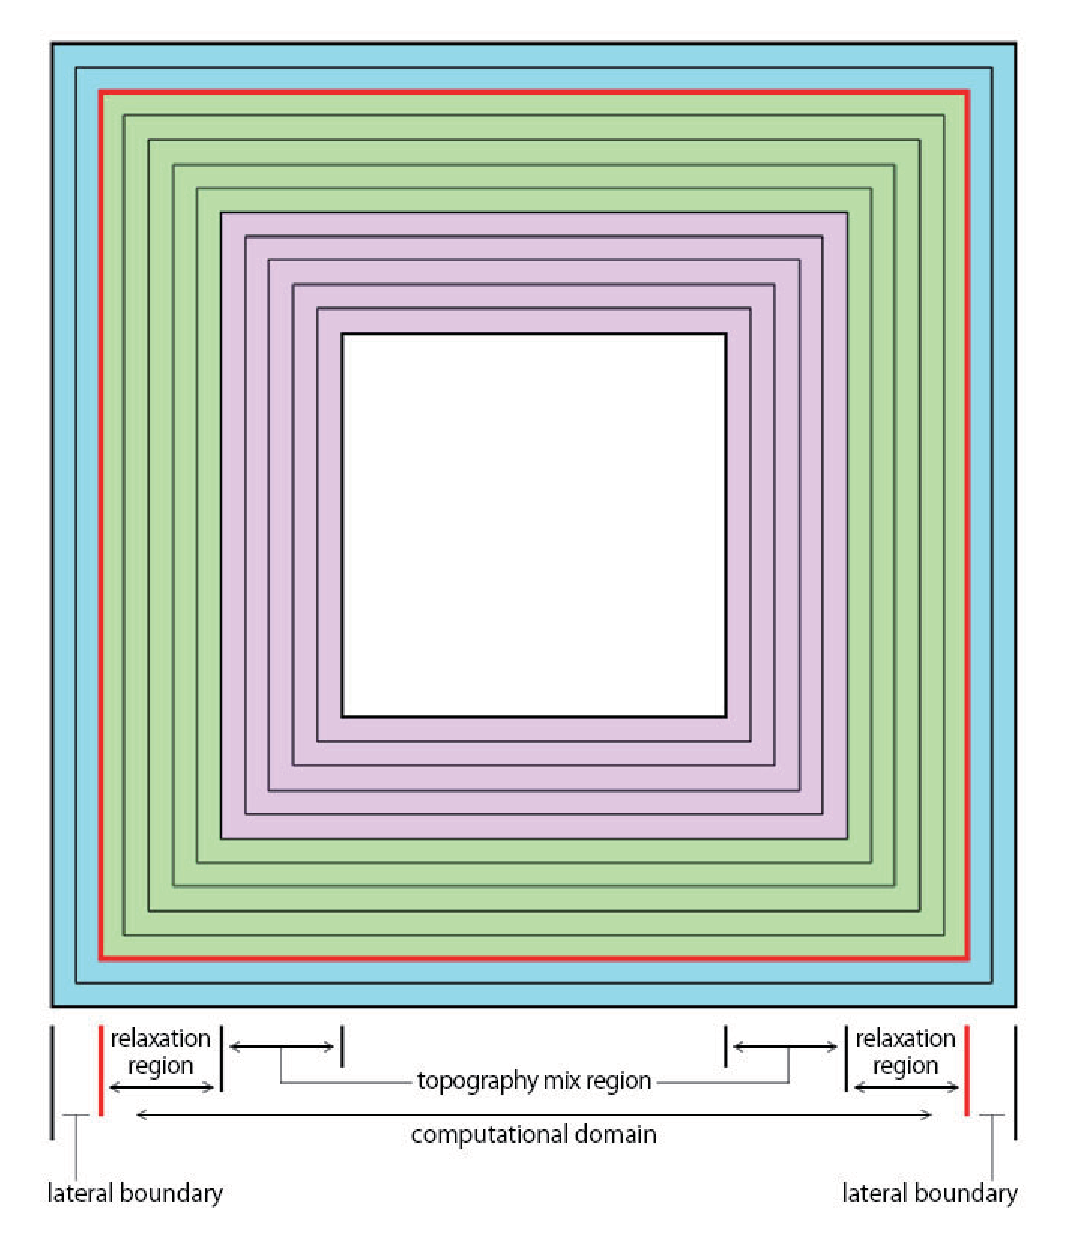
\includegraphics[width=0.4\hsize]{./figure/topo_copy.eps}\\
  \caption{地形コピーを適用した子領域の地形データ水平分布. 最外の水色の2格子(Haloの数。水平差分スキームによって異る)は側面境界で、それより内側の赤色の線で
           囲われた領域が計算領域である。緑色の部分がバッファー領域、桃色の部分が地形遷移領域、そして最内の白色の
           部分が子領域の地形をもつ領域である。地形遷移領域では外側から内側にかけて徐々に親領域の地形データから
           子領域の地形データへ遷移する。}
  \label{fig_topocopy}
\end{center}
\end{figure}

まず親領域の``pp.d01.conf''ファイルを編集して、計算領域の大きさを子領域へ伝えるために緯度経度カタログ
ファイルを出力するように設定する。具体的には、下記の記述を``pp.d01.conf''ファイルに追記する。\\

\noindent {\small {\gt
\ovalbox{
\begin{tabularx}{140mm}{l}
\verb|&PARAM_DOMAIN_CATALOGUE| \\
\verb| DOMAIN_CATALOGUE_FNAME  = "latlon_domain_catalogue.txt",| \\
\verb| DOMAIN_CATALOGUE_OUTPUT = .true.,| \\
\verb|/| \\
\end{tabularx}
}}}\\

\noindent その他の設定項目は通常通りで良い。編集ができたら親領域の地形データ作成を実行する(つまり、
scale-rm\_ppを実行する)。ここで、出力データは、``topo\_d01.pe***.nc''というファイル名で保存されていると
想定する。次に、子領域の``pp.d02.conf''ファイルを編集する。\\

\noindent {\small {\gt
\ovalbox{
\begin{tabularx}{140mm}{l}
\verb|&PARAM_CNVTOPO| \\
\verb|     〜 中略 〜|\\
\verb| CNVTOPO_copy_parent     = .true.,| \\
\verb|/| \\
 \\
\verb|&PARAM_COPYTOPO| \\
\verb| COPYTOPO_IN_BASENAME   = "topo_d01",| \\
\verb| COPYTOPO_ENTIRE_REGION = .false.,| \\
\verb| COPYTOPO_LINEAR_H      = .true.,| \\
\verb|/| \\
 \\
\verb|&PARAM_NEST| \\
\verb| USE_NESTING               = .true.,| \\
\verb| OFFLINE                   = .true.,| \\
\verb| OFFLINE_PARENT_PRC_NUM_X  = 4,| \\
\verb| OFFLINE_PARENT_PRC_NUM_Y  = 4,| \\
\verb| OFFLINE_PARENT_KMAX       = 35,| \\
\verb| OFFLINE_PARENT_IMAX       = 40,| \\
\verb| OFFLINE_PARENT_JMAX       = 40,| \\
\verb| OFFLINE_PARENT_LKMAX      = 5,| \\
\verb| LATLON_CATALOGUE_FNAME    = "latlon_domain_catalogue.txt",| \\
\verb|/| \\
\end{tabularx}
}}}\\

\noindent もともと設定ファイルにある\verb|PARAM_CNVTOPO|の項目に、\verb|CNVTOPO_copy_parent = .true.|
という記述を加える。これは地形コピーの実行を指示するスイッチである。
次の\verb|PARAM_COPYTOPO|は、地形コピーの設定項目群であり、すべて追記すること。
1つ目の\verb|COPYTOPO_IN_BASENAME|は、親領域の地形データのPATHを指定する。ここでは、親領域の
出力データは``topo\_d01.pe***.nc''というファイル名でカレントディレクトリに保存されていると指定している。
2つ目の\verb|COPYTOPO_ENTIRE_REGION|は、全領域でコピーするかどうかを決定するオプションである。
このスイッチをtrueにすると、図\ref{fig_topocopy}に示された桃色と白色の領域は無くなり、全て緑色の
完全コピー領域になる。3つ目の\verb|COPYTOPO_LINEAR_H|は、地形遷移領域の遷移具合を調整するスイッチである。
\verb|COPYTOPO_LINEAR_H|がtrueだと線形プロファイルで遷移し、falseだと指数関数プロファイルで遷移する。

地形遷移領域の幅は、デフォルト設定ではバッファー領域と同じ幅になる。バッファー領域の設定と同じ要領で、
\verb|COPYTOPO_TRANSITION_DX|、\verb|COPYTOPO_TRANSITION_DY|、および\verb|COPYTOPO_TRANSFACT|の
変数を使って任意の幅に設定することができる。

最後の\verb|PARAM_NEST|の項目はオフライン・ネスティング実験のフレームワークを利用するための設定項目であり、
全て追記する必要がある。設定変数の詳しい説明は、\ref{sec:nest_offline}節のオフライン・ネスティング実験の説明を
参照してほしい。

設定ファイルの編集が終われば、子領域の地形データ作成を実行する。3つ以上の領域がある場合は、
上記の実行過程を外側領域から順に繰り返せばよい。



